\begin{activity} \label{A:5.1.3}  
Suppose that $g$ is given by the graph at left in Figure~\ref{F:5.1.Act3} and that $A$ is the corresponding integral function defined by $A(x) = \int_1^x g(t) \, dt$.
\begin{figure}[h]
\begin{center}
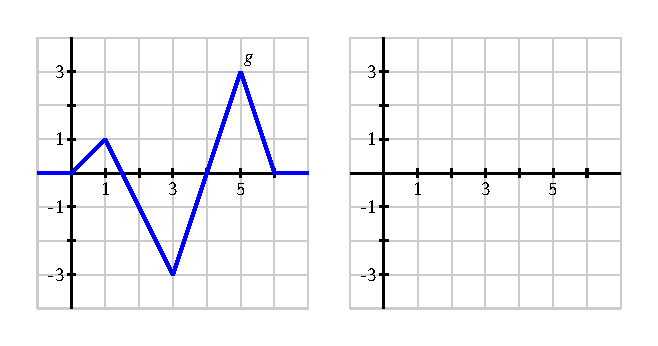
\includegraphics{figures/5_1_Act3.eps}
\caption{At left, the graph of $y = g(t)$; at right, axes for plotting $y = A(x)$, where $A$ is defined by the formula $A(x) = \int_1^x g(t) \, dt$.} \label{F:5.1.Act3}
\end{center}
\end{figure}
\ba
	\item On what interval(s) is $A$ an increasing function?  On what intervals is $A$ decreasing?  Why?
	\item On what interval(s) do you think $A$ is concave up?  concave down?  Why?
	\item At what point(s) does $A$ have a relative minimum?  a relative maximum?
	\item Use the given information to determine the exact values of $A(0)$, $A(1)$, $A(2)$, $A(3)$, $A(4)$, $A(5)$, and $A(6)$.
	\item Based on your responses to all of the preceding questions, sketch a complete and accurate graph of $y = A(x)$ on the axes provided, being sure to indicate the behavior of $A$ for $x < 0$ and $x > 6$.
	\item How does the graph of $B$ compare to $A$ if $B$ is instead defined by $B(x) = \int_0^x g(t) \, dt$?
\ea

\end{activity}
\begin{smallhint}
 \ba
	\item Where is $A$ accumulating positive signed area?	
	\item As $A$ accumulates positive or negative signed area, where is the rate at which such area is accumulated increasing?
	\item Where does $A$ change from accumulating positive signed area to accumulating negative signed area?
	\item Note, for instance, that $A(2) = \int_1^2 g(t) \, dt$.
	\item Use your work in (a)-(d) appropriately.
	\item What is the value of $B(0)$?  How does this compare to $A(0)$?
\ea
\end{smallhint}
\begin{bighint}
 \ba
	\item Where is $A$ accumulating positive signed area? Where is $A$ accumulating negative signed area?
	\item As $A$ accumulates positive or negative signed area, where is the rate at which such area is accumulated increasing?  Contrast, for instance, the behavior of $A$ on the intervals $(0,1)$ and $(1,2)$.
	\item Where does $A$ change from accumulating positive signed area to accumulating negative signed area?  From negative to positive?
	\item Note, for instance, that $A(2) = \int_1^2 g(t) \, dt$, $A(0) = \int_1^0 g(t) \, dt$, and particularly that $A(1) = \int_1^1 g(t) \, dt = 0$.
	\item Use your work in (a)-(d) appropriately.
	\item What is the value of $B(0)$?  How does this compare to $A02)$?  What if we compare $B(1)$ and $A(1)$?
\ea
\end{bighint}
\begin{activitySolution}
\ba
	\item $A$ is accumulating positive signed area wherever $g$ is positive, and thus $A$ is increasing on $(0,1.5)$, $(4,6)$;  $A$ is accumulating negative signed area and therefore decreasing wherever $g$ is negative, which occurs on $(1.5,4)$.
	\item Here we want to consider where $A$ is changing at an increasing rate (concave up) or changing at a decreasing rate (concave down).  On $(0,1)$ and $(4,5)$, $A$ is increasing, and we can also see that since $g$ is increasing, $A$ is increasing at an increasing rate.  Similarly, on $(3,4)$ (where $g$ is negative so $A$ is decreasing), since $g$ is increasing it follows that $A$ is decreasing at an increasing rate.  Thus, $A$ is concave up on $(0,1)$ and $(3,5)$.  Analogous reasoning shows that $A$ is concave down on $(1,3)$ and $(5,6)$.
	\item Based on our work in (a), we see that $A$ changes from increasing to decreasing at $x = 1.5$, and thus $A$ has a relative maximum there.  Similarly, $A$ has a relative minimum at $x = 4$.
	\item Using the fact that $g$ is piecewise linear and the definition of $A$, we find that $A(0) = \int_1^0 g(t) \, dt = -\int_0^1 g(t) \, dt = -\frac{1}{2}$; $A(1) = \int_1^1 g(t) \, dt = 0$; $A(2) = \int_1^2 g(t) \, dt = 0$.  Analogous reasoning shows that $A(3) = -2$, $A(4) = -3.5$, $A(5) = -2$, $A(6) = -0.5$.
	\item Use your work in (a)-(d) appropriately.
	\item Note that $B(0) = 0$, while $A(0) = -\frac{1}{2}$.  Likewise, $B(1) = \frac{1}{2}$, while $A(1) = 0$.  Indeed, we can see that for any value of $x$, $B(x) = A(x) + \frac{1}{2}$.
\ea
\end{activitySolution}
\aftera